\documentclass[../report.tex]{subfiles}
\begin{document}
\subsection{Mô hình}
\paragraph*{}
Từ thí nghiệm của Milgram, Kleinberg đã đề xuất một hướng tiếp cận mô hình Small-world có ứng dụng khá lớn vào các hệ thống Datacenter. Thuật toán dựa trên sự kết nối tự nhiên giữa các thực thể là con người với nhau trong một mạng xã hội.
\paragraph*{Đầu vào:} Với một topo theo dạng Grid hoặc Torus cho sẵn G(V, E) với V là tập đỉnh, E là tập cạnh. Cho trước tham số $\alpha$ đóng vai trò là tham số cho xác suất ngẫu nhiên.
\paragraph*{Đầu ra:} Từ tham số ngẫu nhiên $\alpha$, tạo ra đồi thị mới được bổ sung thêm các kết nối dài giữa các điểm trong topo với nhau theo cặp. 
\paragraph*{Phân tích:} Trong thuật toán ta xây dựng một tập các ứng cử viên candidates theo của mỗi node đang xét theo luật:
\begin{itemize}
    \item Node đang xét không thuộc candidates.
    \item Hàng xóm (những node đã có liên kết với node đang xét) không thuộc candidates.
    \item Những node không còn khả năng nhận liên kết thì không thuộc candidates.
\end{itemize}

\paragraph*{Thuật toán}
Với mỗi đỉnh nguồn u trong V ta xét:
\begin{itemize}
    \item Với mỗi đỉnh v trong candidates, xác suất kết nối giữa u và v được định nghĩa như sau: \\
        \begin{equation}
            Pr[u \rightarrow v] \sim D^{-\alpha}(u, v)
        \end{equation}
    \item Từ một giá trị ngẫu nhiên $\triangledown \in$ (0, 1) ta sẽ chọn được đích v là node có nhãn lớn nhất thỏa mãn: 
        \begin{equation}
            \sum Pr[u \rightarrow v] \le \triangledown
        \end{equation}
\end{itemize}

\subparagraph*{Với}
\begin{itemize}
    \item D(u, v) là khoảng cách giữa 2 node u và v (tính theo bước lưới).
    \item Với mỗi node nguồn đang x, tập các đỉnh trong candidates là tập đầy nên:
        \begin{equation}
            1 = \sum Pr[u \rightarrow v] \sim \sum D^{-\alpha}(u, v) = \triangledown
        \end{equation}
        Từ (1) và (2) ta có: 
            \begin{equation}
                Pr[u \rightarrow v] = \triangledown^{-1}.D^{-\alpha}(u, v)
            \end{equation}
\end{itemize}

\subsubsection*{Với topo 2D-Grid}
Bước lưới giữa hai node u($x_1$; $y_1$) và v($x_2$; $y_2$) là: $D(u, v) = |x_1 - x_2| + |y_1 - y_2|$
\subsubsection*{Với topo 2D-Torus}
Với Torus, do có tính \textit{regular} và \textit{symmetric} nên ở đây $\triangledown$ là giống nhau đối với tất cả các node của đồ thị. Và khoảng cách giữa hai node u($x_1$; $y_1$) và v($x_2$; $y_2$) khi đó là $D(u, v) = D_x + D_y$ với:

\par
\[
D_x =  
\left\{
\begin{array}{cc}
|x_2 - x_1|  & |x_2 - x_1| \le \left[\frac{M}{2}\right] \\ \\ 
M - |x_2 - x_1| & |x_2 - x_1| \ge \left[\frac{M}{2}\right]  
\end{array}
\right.
\]

\par
\[
D_y =  
\left\{
\begin{array}{cc}
|y_2 - y_1|  & |y_2 - y_1| \le \left[\frac{N}{2}\right] \\ \\
N - |y_2 - y_1| & |y_2 - y_1| \ge \left[\frac{N}{2}\right]  
\end{array}
\right.
\]

Ta có thể thấy ngay rằng, với tham số xác suất có giá trị càng lớn, sẽ kéo theo giá trị xác xuất kết nối giữa 2 node cũng trở lên càng nhỏ. Do đó, khả năng xuất hiện các kết nối dài cũng ngày càng thấp; thay vào đó, ta sẽ chỉ thấy các kết nối ngắn, và đồ thị sẽ thưa dần ra nếu ta tăng giá trị $\alpha$ lên.
\subsection{Chương trình thực nghiệm}
\paragraph*{Xây dựng 2D-Grid}
Topo Grid được xây dựng dựa trên nhận xét sau:
\begin{itemize}
        \item Bốn node ở 4 góc có bậc là 2
        \item Các node khác 4 node trên mà thuộc hàng(cột) đầu hoặc hàng(cột) cuối cùng thì có bậc là 3
        \item Các node còn lại sẽ có bậc là 4
\end{itemize}

Thủ tục tạo 2D-Grid kích thước r hàng x c cột:
\begin{algorithm}[H]
		\caption{Thuật toán xây dựng topo 2D-Grid kích thước r x c}
		\begin{algorithmic}[1]
            \Procedure{init2DGrid}{$r$, $c$}
			\For {each node $u$ in $V$}
            \If {u.y - 1 $\ge$ 0}
            \State makeLink(u, node(u.y - 1, u.x))
            \EndIf
            \If {u.y + 1 < r}
            \State makeLink(u, node(u.y + 1, u.x))
            \EndIf
            \If {u.x + 1 < c}
            \State makeLink(u, node(u.y, u.x + 1))
            \EndIf
            \If {u.x - 1 $\ge$ 0}
            \State makeLink(u, node(u.y, u.x - 1))
            \EndIf
			\EndFor
			\EndProcedure
		\end{algorithmic}
\end{algorithm}
\begin{figure}[H]
    \centering
    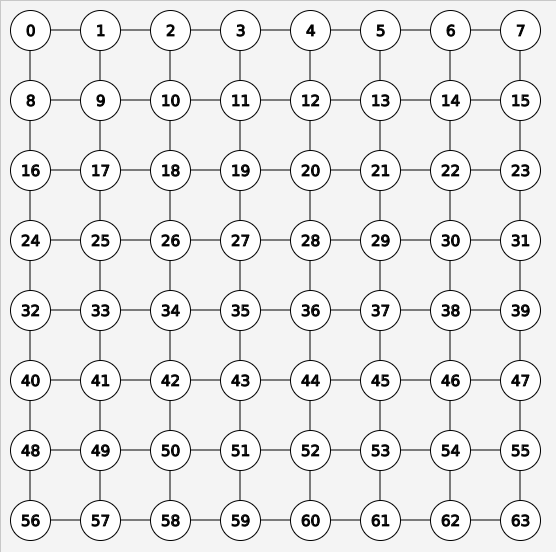
\includegraphics[scale=0.41]{figures/grid.png}
    \caption {Grid 2D kích thước 8x8}
\end{figure}

\paragraph*{Xây dựng 2D-Torus}
Với topo 2D-Torus thì do tính đối xứng, nên mỗi node trong mạng đều có bậc là 4.
Do vậy thủ tục để tạo nên topo 2D-Torus ban đầu sẽ tạo nên các liên kết của topo Grid, sau đó sẽ tạo thêm các liên kết ở các node mà chưa đạt được bậc là 4 theo thủ tục sau:
\begin{algorithm}[H]
		\caption{Thuật toán xây dựng topo 2D-Torus kích thước r x c}
		\begin{algorithmic}[1]
            \Procedure{paddingLink}{$r$, $c$}
			\For {each node $u$ in $V$}
            \If {u.y - 1 < 0}
            \State makeLink(u, node(c + u.y - 1, u.x))
            \EndIf
            \If {u.y + 1 $\ge$ r}
            \State makeLink(u, node(u.y + 1 - r, u.x))
            \EndIf
            \If {u.x + 1 $\ge$ c}
            \State makeLink(u, node(u.y, u.x + 1 - c))
            \EndIf
            \If {u.x - 1 < 0}
            \State makeLink(u, node(u.y, u.x - 1 + c))
            \EndIf
			\EndFor
			\EndProcedure
		\end{algorithmic}
\end{algorithm}
\begin{figure}[H]
    \centering
    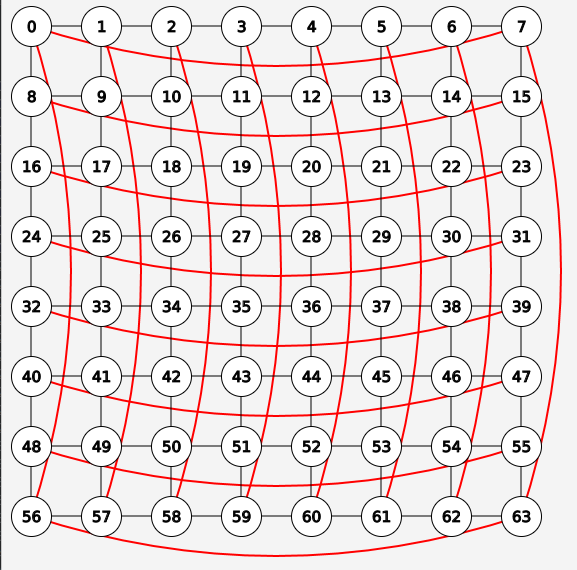
\includegraphics[scale=0.5]{figures/torus.png}
    \caption {Torus 2D kích thước 8x8}
\end{figure}
\paragraph*{Kết quả}
Sau khi đã xây dựng được topo gốc chúng ta sẽ tiến hành cài đặt thuật toán trên mỗi topo. Một số kết quả thu được sau khi chạy thực nghiệm:

\begin{figure}[H]
    \centering
    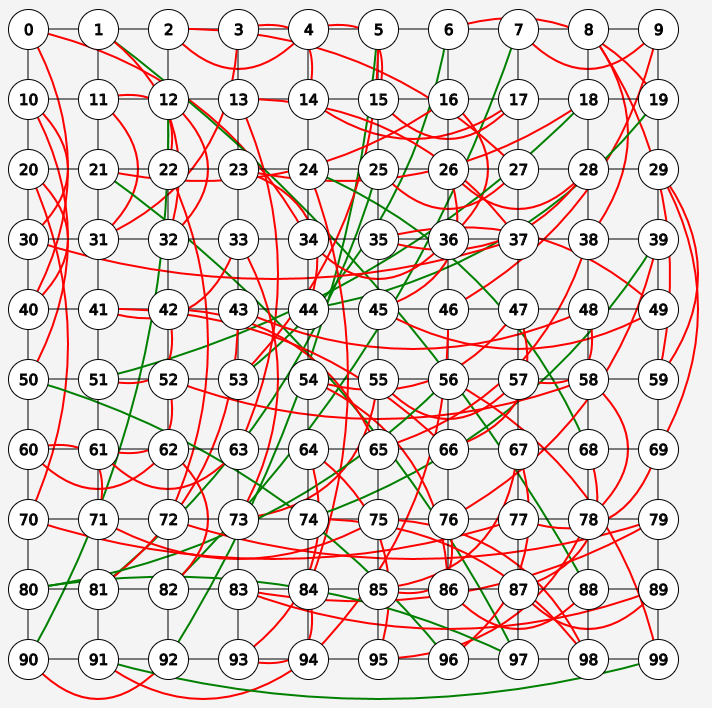
\includegraphics[scale=0.55]{figures/grid16.png}
    \caption{Small world 2D-Grid với $\alpha$ = 1.6}
\end{figure}

\begin{figure}[H]
    \centering
    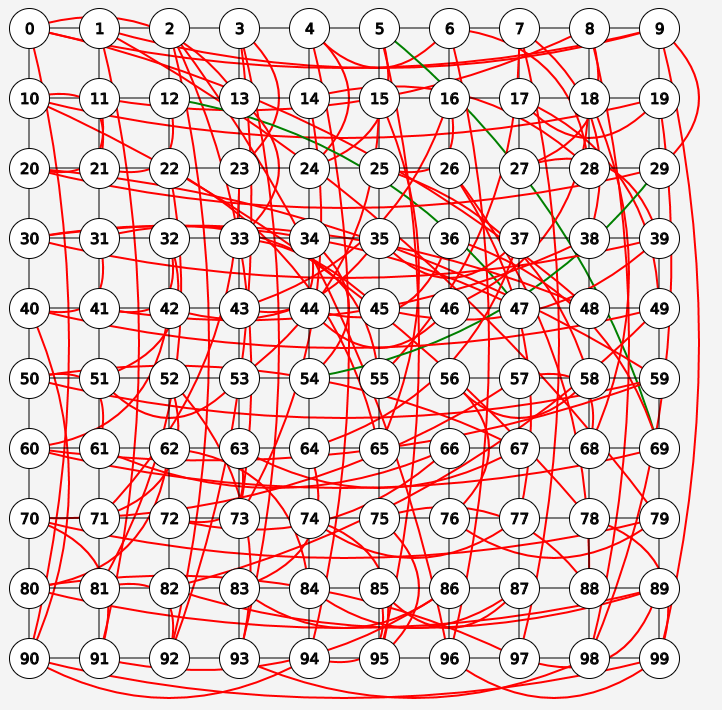
\includegraphics[scale=0.55]{figures/torus16.png}
    \caption{Small world 2D-Torus với $\alpha$ = 1.6}
\end{figure}

\begin{figure}[H]
    \centering
    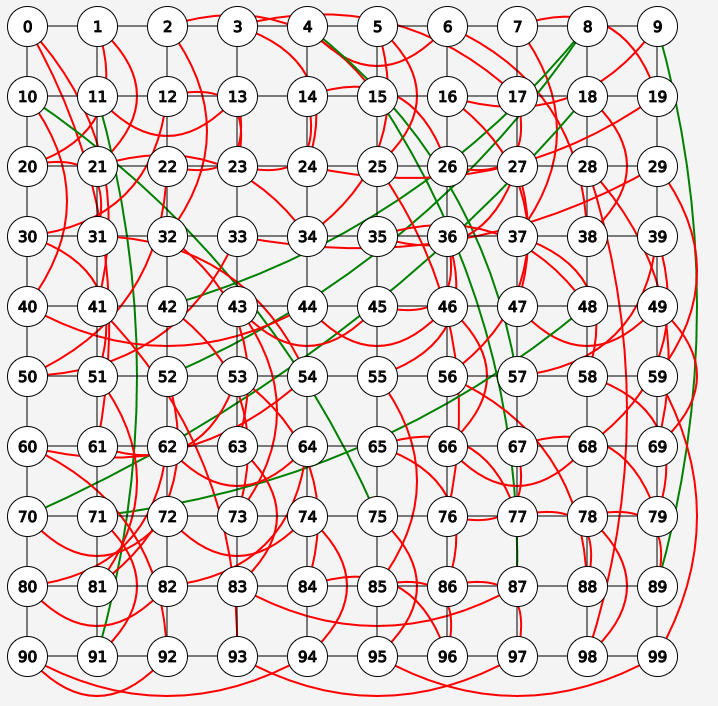
\includegraphics[scale=0.55]{figures/grid2.png}
    \caption{Small world 2D-Grid với $\alpha$ = 2}
\end{figure}

\begin{figure}[H]
    \centering
    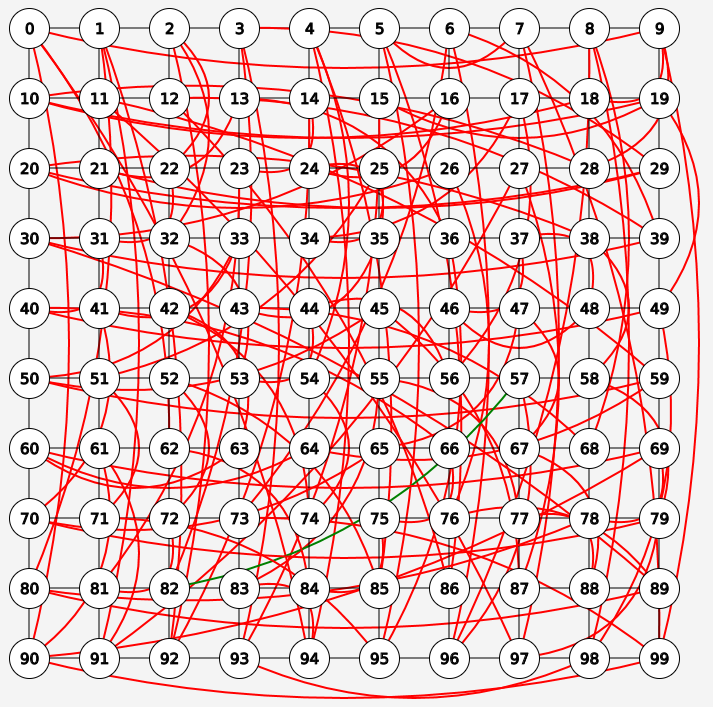
\includegraphics[scale=0.55]{figures/torus2.png}
    \caption{Small world 2D-Torus với $\alpha$ = 2}
\end{figure}

\end{document}
